\documentclass[UTF8]{ctexart}
\usepackage{graphicx}

\usepackage{geometry}
\geometry{papersize={20cm, 15cm}}
\geometry{left=1cm, right=2cm, top=3cm, bottom=4cm}

\title{論文標題}
\author{Bing}
\date{\today}

\usepackage{setspace}
\onehalfspacing

\addtolength{\parskip}{.4em}

\usepackage{fancyhdr}
\pagestyle{fancy}
\lhead{\date}
\renewcommand{\headrulewidth}{0.4pt}
\renewcommand{\headwidth}{\textwidth}

%start
\begin{document}
\maketitle
hello world

\section{section}
文字。
\subsection{subsection}

\[ \{abcdef\} \]

\subsubsection{subsubsection}
    根據Robot Framework \cite{pa}
\paragraph{paragraph}
    \normalsize\textsf{粗體文字}
    \Large 大文字
    
\subparagraph{subparagraph}
文字
    \begin{figure}[htbp]
    \centering
    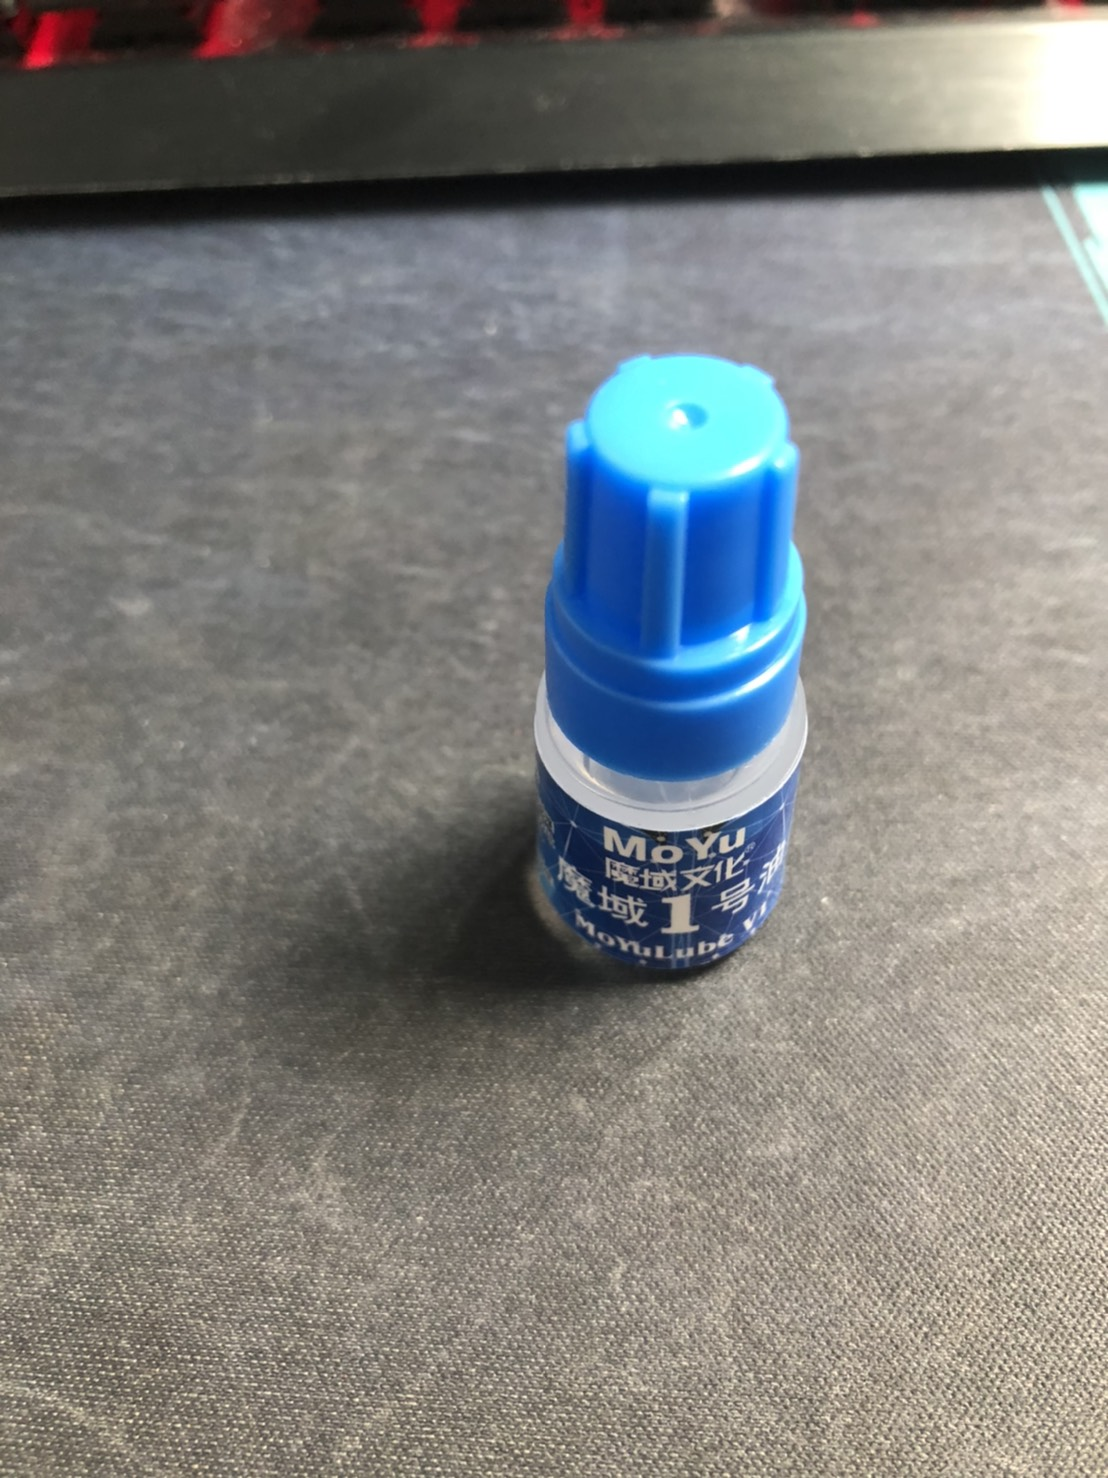
\includegraphics[width= .1\textwidth]{test.jpg}
    \caption{圖片測試}
    % \label{fig:myphoto}
    \end{figure}

    \begin{figure}[htbp]
    \centering
        \begin{tabular}{|c|||}
        \hline
        代理關鍵字類别 \\
        \hline
        1.AlertShouldBePresentProxy \\
        \hline
        2.CountValuesInListProxy \\
        \hline
        \end{tabular}
    \caption{本論文新增的20種代理關鍵字類別}
    \end{figure}

    \begin{thebibliography}{100}
        \bibitem{pa} example reference here(1996)
    \end{thebibliography}

\end{document}

